\documentclass[../slides.tex]{subfiles}
\begin{document}

\begin{frame}{Gliederung}
  \begin{minipage}[]{.49\textwidth}
    \begin{block}{Themen}
      \begin{itemize}
          \item Additive Fertigung
          \item Digitalisierung von Bauteilen
          \item Optische Spannkraftdeformationsanalyse
          \item Automatisierung 
          \item Ausblick
      \end{itemize}
    \end{block}
  \end{minipage}
  \hfill
  \begin{minipage}[]{.49\textwidth}
    \begin{figure}[]
      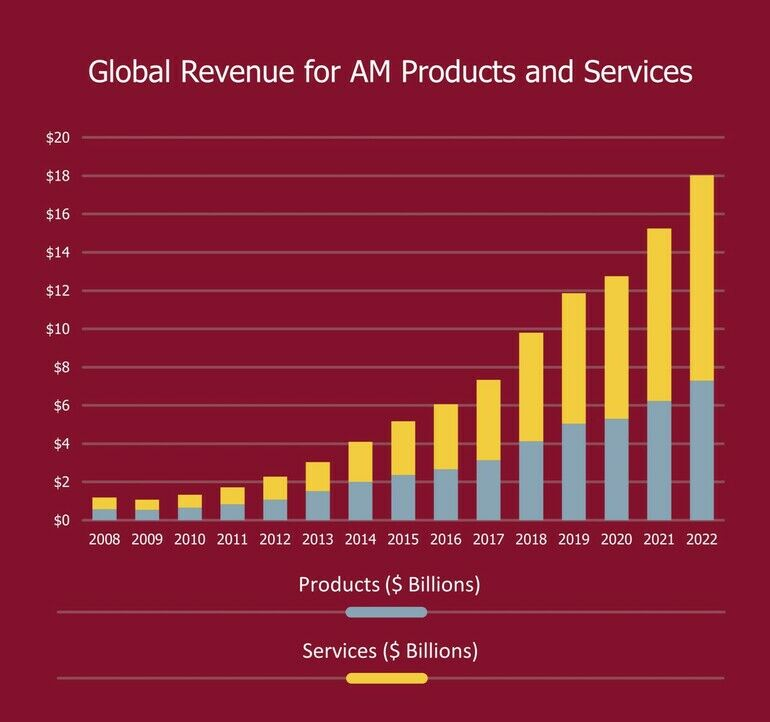
\includegraphics[height=165pt]{img_niklas/Picture3-1-scaled_0FB63A00-D319-40EF-A648-9739A68215D6.jpg}
      \caption{\tiny{\url{https://additive.industrie.de/news/wohlers-report-2023-additive-fertigung-legt-um-183-zu/} (07.03.2024)\\}}
      \label{fig:globalRev}
      %https://additive.industrie.de/news/wohlers-report-2023-additive-fertigung-legt-um-183-zu/
    \end{figure}
  \end{minipage}
\end{frame}

\begin{frame}{Additive Fertigung: Verfahren SLM und FDM}
  \begin{minipage}[]{0.49\textwidth}
    \begin{figure}[]
      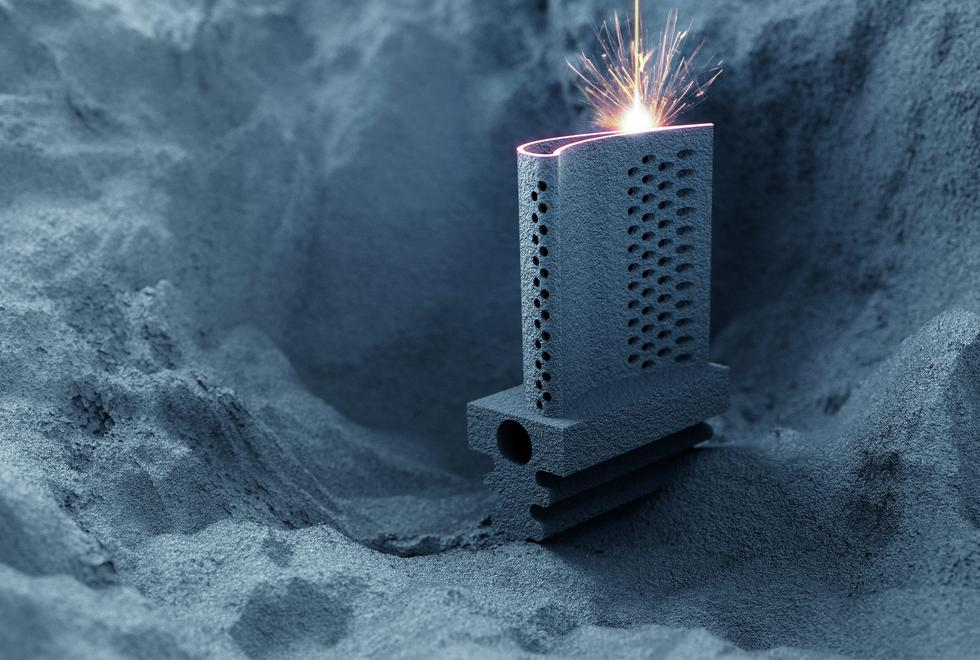
\includegraphics[width=150pt]{img_niklas/csm_h_bearb_LASERTEC_SLM_Blade_Powder_e24c562ac8.jpg}
      \caption{Selective Laser Melting \\ \tiny{\url{https://www.wdoose.de/en/additive-fertigung/slm-selective-laser-melting/} (07.03.2024)}}
      \label{fig:slm}
    \end{figure}
  \end{minipage}
  \begin{minipage}[]{0.49\textwidth}
    \begin{figure}[]
      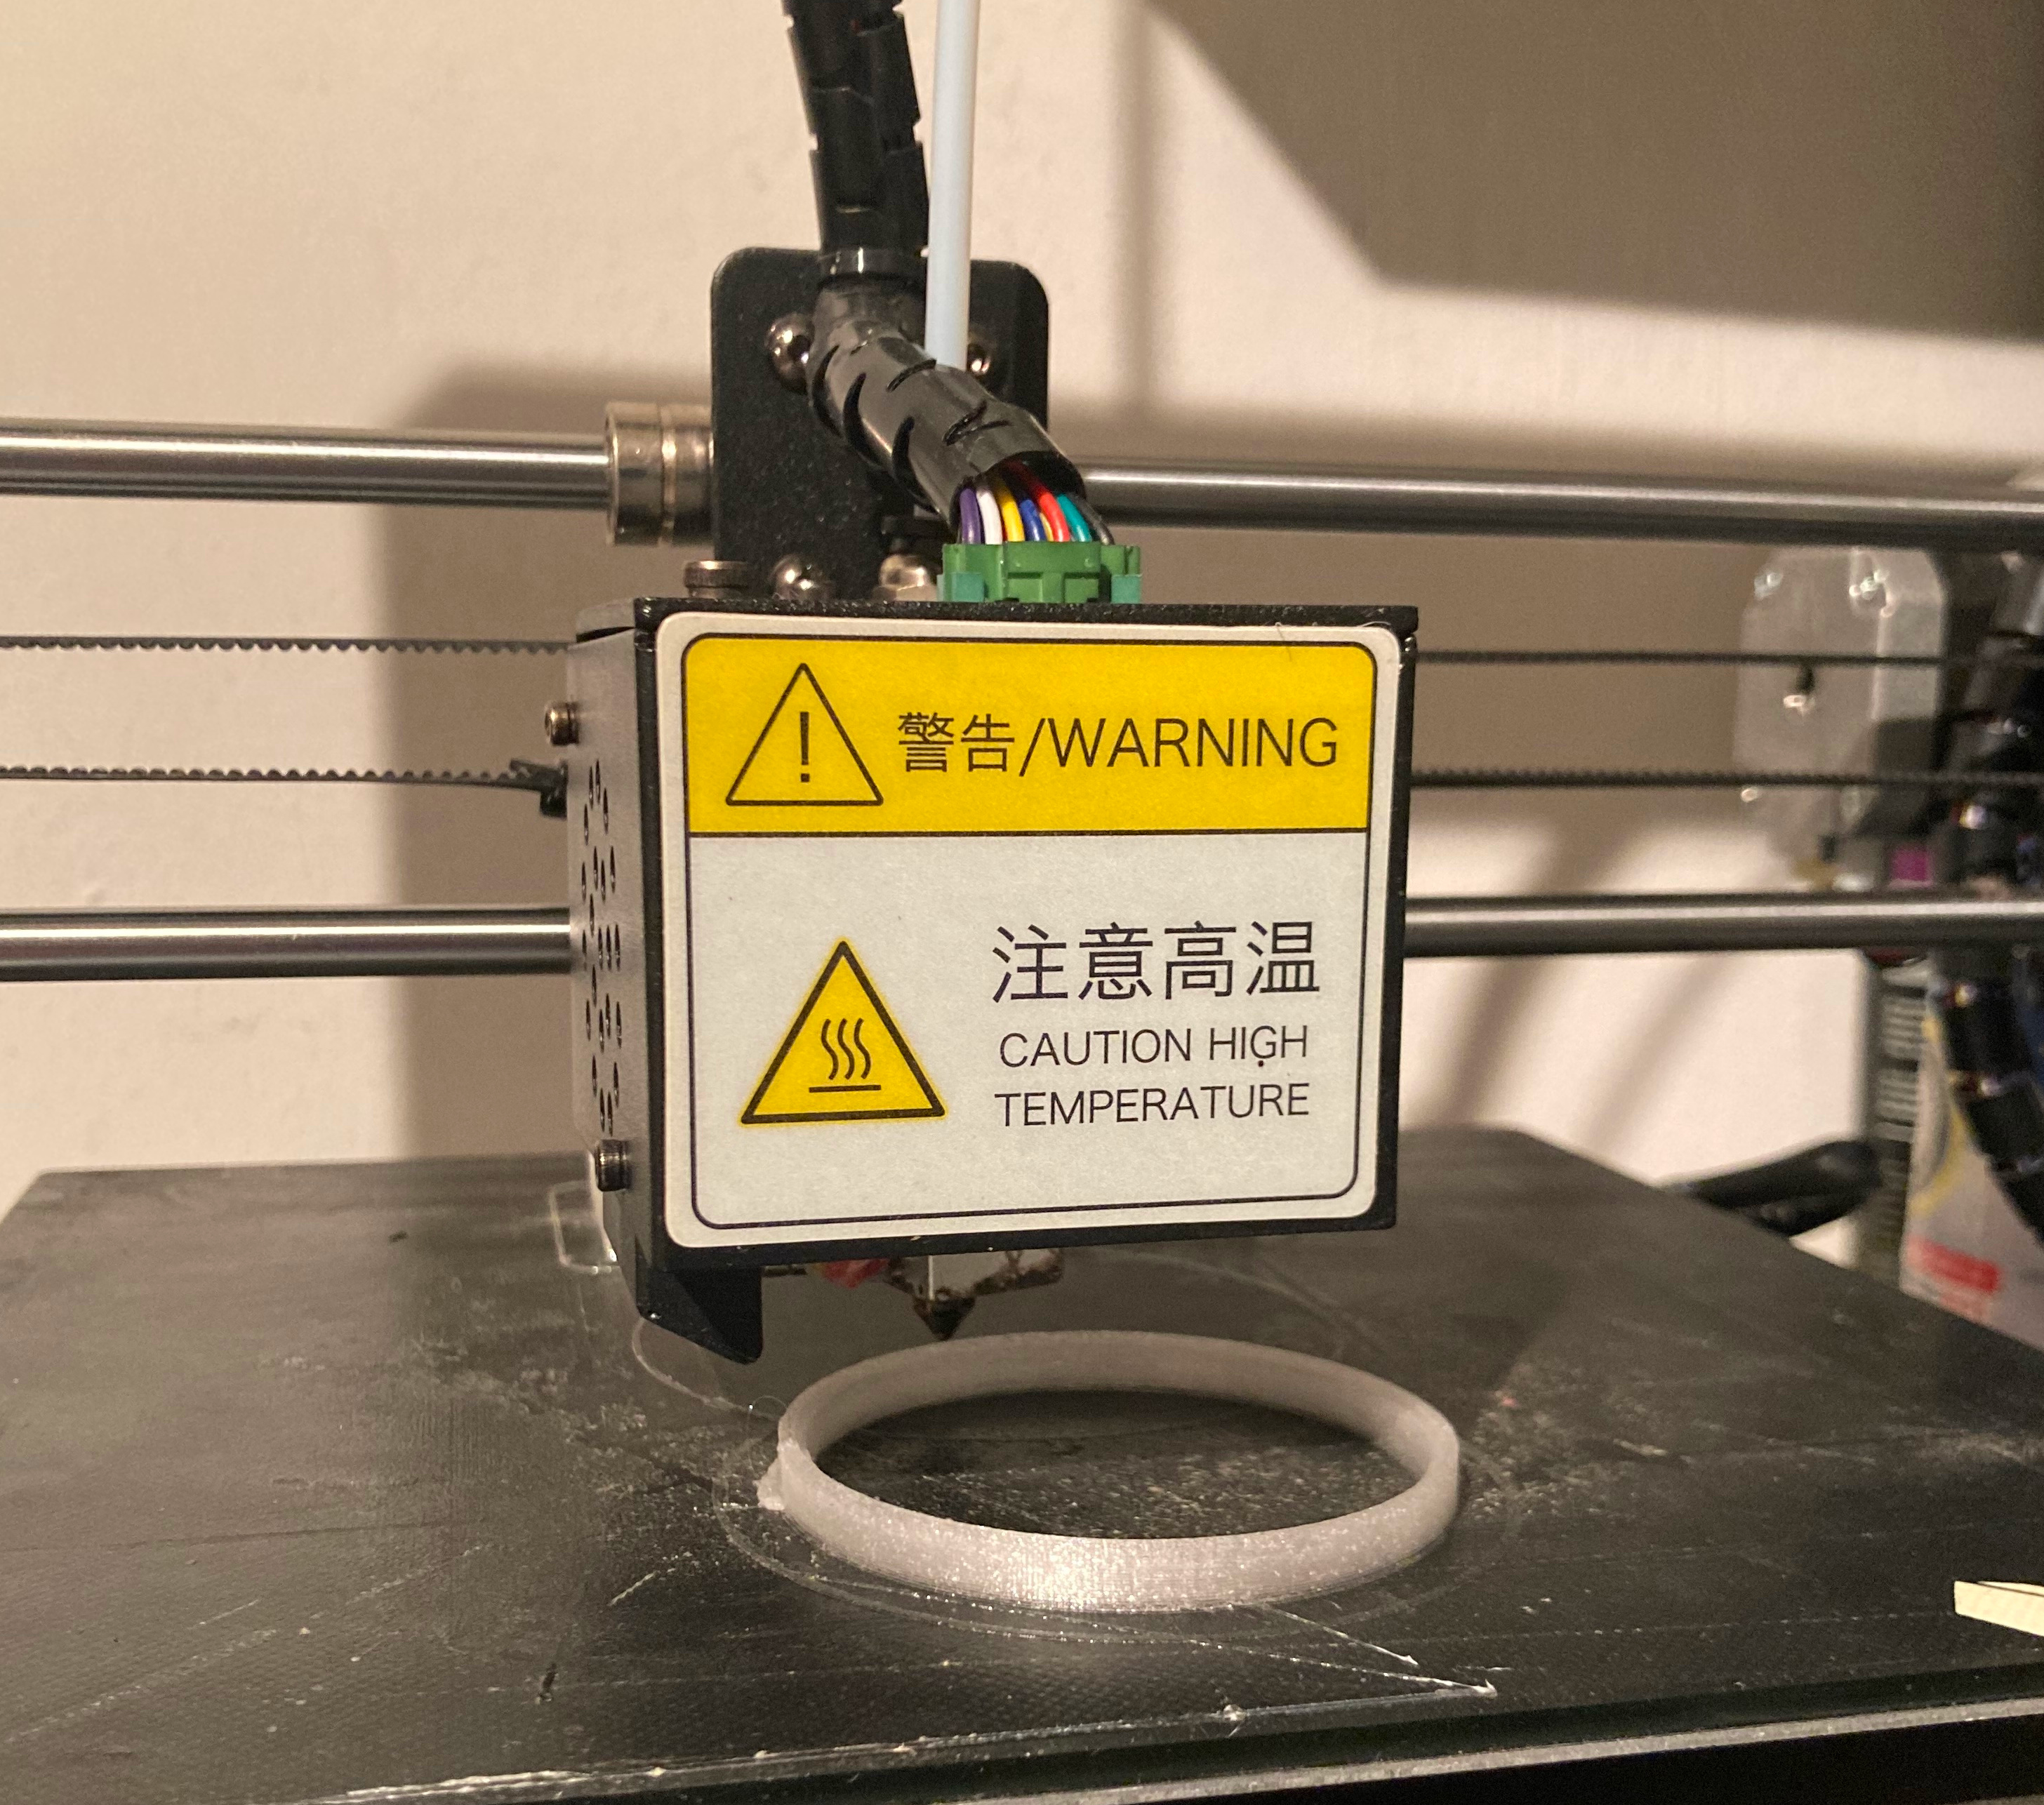
\includegraphics[height=140pt]{img_niklas/3d_printer.jpg}
      \caption{Fused Deposition Modeling}
    \end{figure}
  \end{minipage}
\end{frame}

\begin{frame}{Additive Fertigung: Limitierungen und Post-Processing}
  \begin{minipage}[t]{\textwidth}
    \begin{figure}[]
      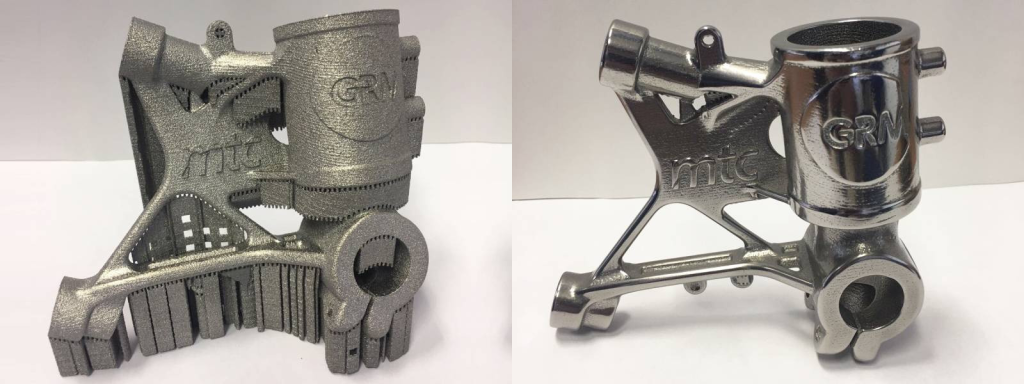
\includegraphics[width=\textwidth]{img_niklas/image-32-1024x384.png}
      \caption{\tiny{\url{https://www.unionfab.com/blog/2023/08/post-processing-methods-metal-3d-printing} (07.03.2024)}}
      \label{fig:post_processing}
    \end{figure}
  \end{minipage}
\end{frame}

\begin{frame}{Einspannen und Nachbearbeiten}
  \begin{figure}[]
      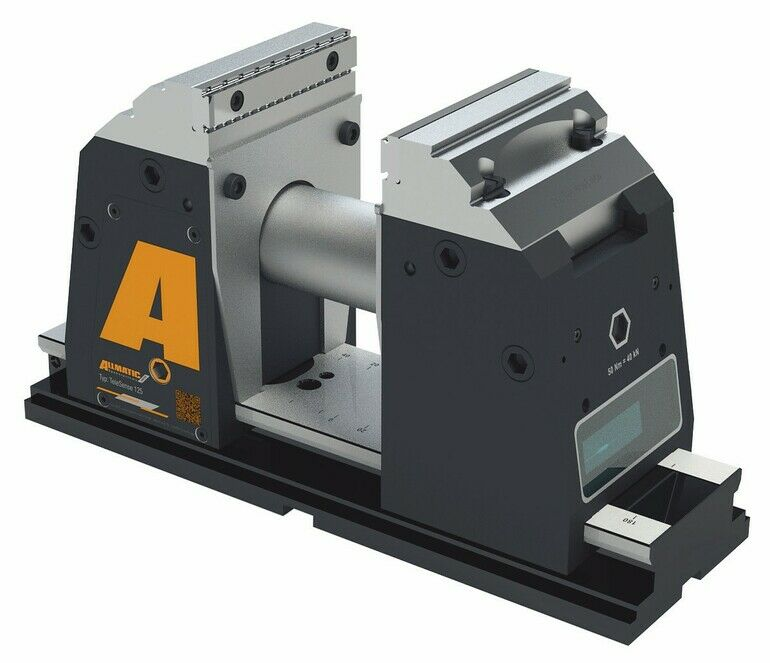
\includegraphics[height=\textheight-70pt]{img_niklas/TeleSense_mit_Backen_final_93BB1CAF-5AC9-467B-ABD7-22EEFC24189A.jpg}
      \caption{Schraubstock mit Spannkraftüberwachung \\ \tiny{\url{https://mav.industrie.de/werkzeuge/innovativer-schraubstock-vereinfacht-5-achs-bearbeitung/}}(07.03.2024)}
      \label{fig:schraubstock}
      %https://mav.industrie.de/werkzeuge/innovativer-schraubstock-vereinfacht-5-achs-bearbeitung/#slider-intro-1
    \end{figure}
    
\end{frame}


\begin{frame}{Optische Spannkraftdeformationsanalyse}
  \begin{minipage}[]{0.6\textwidth}
    \begin{block}{Ziel}
      \begin{itemize}
        \item Automatische Erkennung von Bauteildeformation 
      \end{itemize}
    \end{block}
    \begin{block}{Arbeitsschritte}
      \begin{itemize}
        \item Digitalisierung des Bauteils
        \item Entwicklung der Stitching-Methodik
        \item Benchmarking an Demonstratorbauteil
        \item Entwicklung der automatisierten Deformationserkennung
        \item Validierung der Methodik an unterschiedlichen Bauteilgeometrien
      \end{itemize}
    \end{block}
  \end{minipage}
  \begin{minipage}[]{0.39\textwidth}
    \begin{figure}[]
      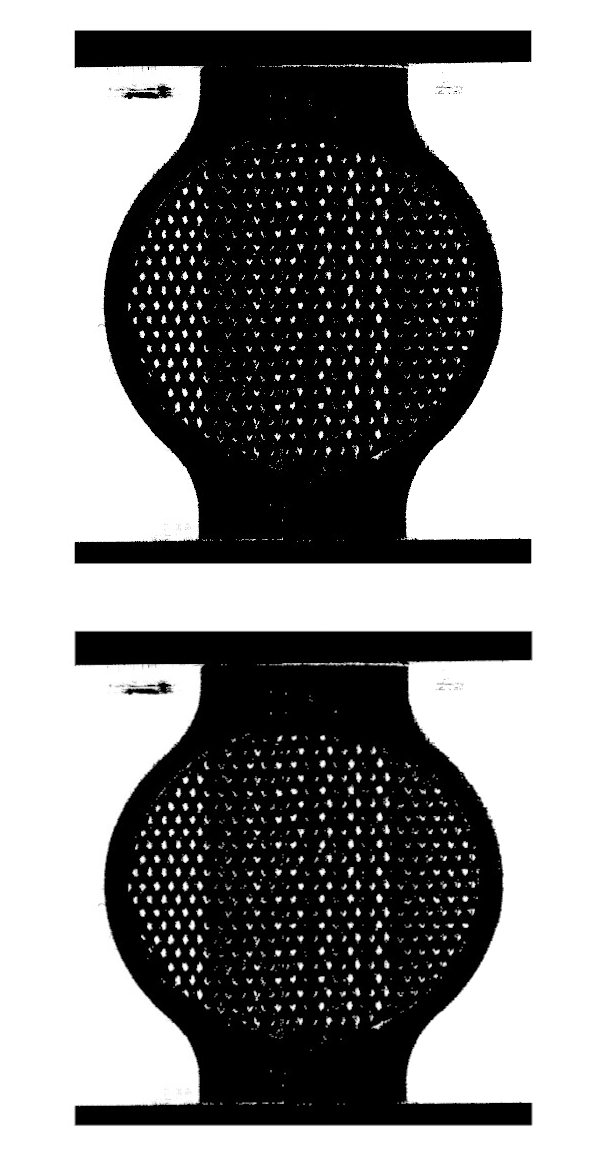
\includegraphics[height=170pt]{img_niklas/compare.png}
      \caption{Vergleich}
    \end{figure}
  \end{minipage}
\end{frame}

\begin{frame}{Demonstratorbauteil}
  \begin{minipage}[h]{.49\textwidth}
    \begin{figure}[]
      
\includegraphics[width=150pt]{img_niklas/base_image.png}
      \caption{STL des Demonstratorbauteils}
      %
    \end{figure}
  \end{minipage}
  \hfill
  \begin{minipage}[h]{.49\textwidth}
    \begin{figure}[]
      
\includegraphics[width=150pt]{img_niklas/base_top_down.png}
      \caption{TOP-DOWN Ansicht (generiert)}
      %
    \end{figure}
  \end{minipage}
\end{frame}

\end{document}